\documentclass[11pt]{article}
\usepackage[margin=0.86in]{geometry}
\usepackage[T1]{fontenc}
\usepackage[utf8]{inputenc}
\usepackage{microtype}
\usepackage{graphicx}
\usepackage{booktabs}
\usepackage{array}
\usepackage{tabularx}
\usepackage{float}
\usepackage{enumitem}
\usepackage{amsmath}
\usepackage{hyperref}
\hypersetup{colorlinks=true,linkcolor=blue,citecolor=blue,urlcolor=blue,pdftitle={Qualifying Image-Grounded Tag Retrieval in Piping and Instrumentation Diagrams with Source-Isolated Counterfactual Evaluation}}
\graphicspath{{figures/}}
\setlength{\emergencystretch}{3em}
\newcolumntype{Y}{>{\raggedright\arraybackslash}X}
\newcolumntype{P}[1]{>{\raggedright\arraybackslash}p{#1}}

\title{Qualifying Image-Grounded Tag Retrieval in Piping and Instrumentation Diagrams with Source-Isolated Counterfactual Evaluation}
\author{Author names and affiliations to be supplied at submission}
\date{}

\begin{document}
\maketitle

\begin{abstract}
Engineering use of vision--language model outputs requires qualification of a
specific task, budget, and drawing family rather than reliance on aggregate
accuracy. We present SABER-PID, a source-isolated, answer-hidden,
counterfactual workflow for candidate-tag retrieval from piping and
instrumentation diagrams (P\&IDs). On 100 unseen PIDQA drawings, frozen
Qwen3-VL-8B at 3072-side produced tag F1 0.5549; source-shuffled and no-image
controls reduced F1 to 0.0062 and 0. At a common 512-token cap, the
3072-minus-768 visual-budget effect was +0.5250 (95\% source-bootstrap interval
[0.4224, 0.6293]). A 54-cell extension across two Qwen scales, InternVL3.5-8B,
three source-disjoint subsets, and two prompts yielded positive lower bounds
for all 36 controls. At the closest safe 54-tile budget, InternVL pooled
correct-image F1 reached 0.4846 and its correct-minus-shuffled effect was
+0.4715 ([0.4064, 0.5332]). At the qualified 3072/512 budget, clean, JPEG, mild blur, and
downsampled images retained pooled correct-minus-shuffled effects of
0.548--0.575; all quality-minus-clean intervals included zero. On a second
public DEXPI family (35 images, 65 questions), Qwen reached precision 0.9231,
recall 0.8889, and F1 0.9057, versus zero F1 under cross-case shuffling and no
image. OCR and Qwen were complementary on PIDQA: union reached recall 0.7040
and F1 0.6339, whereas intersection reached precision 0.9907. The
cost-sensitive lower envelope selects intersection, joined OCR, OCR-first, or
union as missed-tag cost increases. SABER-PID therefore supports configurable,
image-grounded candidate-tag retrieval under the evaluated PIDQA and DEXPI
conditions; it does not qualify topology reasoning or field deployment.
\end{abstract}

\noindent\textbf{Keywords:} engineering document intelligence; vision--language
models; optical character recognition; tag retrieval; source isolation;
counterfactual evaluation

\section{Introduction}

Piping and instrumentation diagrams encode equipment, instruments, process
lines, and control relationships in visually dense engineering documents.
Their identifiers connect drawings to equipment lists, maintenance records,
and engineering databases. Candidate-tag retrieval is therefore useful for
document indexing, search, and migration even when full graph reconstruction
is not yet available.

The central deployment question is not simply whether a multimodal model
obtains a high score. A model can exploit answer priors, repeated drawing
identity, or task regularities; small text may also disappear under an
insufficient visual-input budget. In our benchmark, aggregate strict accuracy
illustrates this problem directly: the task-prior diagnostic scores 0.3375,
the no-image condition 0.3025, and the correct-image condition 0.2875.
Aggregate accuracy therefore cannot by itself qualify image reading. A useful
engineering evaluation must instead test whether a task-specific effect
follows the requested drawing, survives a matched output budget, and remains
within explicitly stated scope boundaries.

Prior P\&ID work has emphasized symbol and text recognition, line extraction,
graph conversion, and end-to-end digitization
\cite{rahul2019,paliwal2021,kim2021,su2024}. PIDQA contributes 64,000
graph-derived questions from 500 synthetic source sheets
\cite{gupta2025}. This resource enables controlled multimodal evaluation but
also creates dependence: many records share the same drawing. Question-random
splitting can therefore expose source-specific information unavailable on an
unseen drawing, a grouped-data failure addressed by multiple-source
cross-validation and leakage-aware evaluation
\cite{geras2013,kapoor2023}.

Document VQA studies likewise distinguish answer similarity from document
groundedness \cite{mathew2021,nourbakhsh2025}. Counterfactual VQA research
uses altered visual or textual evidence to expose shortcut dependence
\cite{chen2020}; large-VLM studies show that fluent predictions may remain
unsupported by the visual input \cite{li2023pope,leng2024}. These findings
motivate an engineering qualification view: a capability is accepted only
for the task, model, budget, and source family for which its evidence gates
pass.

We call this workflow \emph{SABER-PID}: source-isolated, answer-hidden,
budget-recorded, evidence-counterfactual, and reported-by-task evaluation. It
is an evaluation and decision workflow, not a new model architecture. The
contributions are:

\begin{enumerate}[leftmargin=1.5em,itemsep=2pt]
\item a source-level qualification contract that separates aggregate
diagnostics from the candidate-tag retrieval claim;
\item paired correct-image, source-shuffled-image, no-image, and matched-budget
contrasts on answer-hidden manifests;
\item pooled and source-macro estimators, source-cluster uncertainty,
TP/FP/FN accounting, and per-drawing candidate workload;
\item a complete family of reference-free OCR--VLM operating modes, a
cost-sensitive deployment rule, and overlap-audited frozen-rule checks that
distinguish initial description from later stability evidence.
\end{enumerate}

\section{Related work and evaluation objective}

\subsection{P\&ID recognition and engineering information extraction}

Classical P\&ID digitization pipelines decompose recognition into symbols,
text, lines, associations, and graph construction
\cite{rahul2019,paliwal2021}. Kim et al. developed symbol and text recognition
for high-density industrial diagrams \cite{kim2021}; Su et al. combined
symbol, text, and pipeline recognition on high-resolution industrial drawings
\cite{su2024}. More recent work demonstrates why raw OCR is only an
intermediate layer: engineering identifiers require format-aware validation
and semantic interpretation \cite{shteriyanov2026}. Our target is narrower
than end-to-end digitization. We evaluate retrieval of candidate value tags
from a complete drawing and do not infer connectivity or topology.

\subsection{Document VQA, grounding, and grouped evaluation}

DocVQA and ChartQA established document-oriented question answering as a
joint text, layout, and reasoning problem \cite{mathew2021,masry2022}.
Grounding-aware evaluation asks whether an answer can be attributed to the
input document rather than only whether its surface form matches a reference
\cite{nourbakhsh2025}. Counterfactual samples and contrastive controls expose
visual and linguistic shortcuts \cite{chen2020,leng2024}. Separately,
multiple-source cross-validation requires related observations to remain in
one partition \cite{geras2013}. SABER-PID combines these ideas as a
measurement contract: drawings are the resampling and splitting unit,
references are hidden from inference, and image identity is intervened on
directly.

\subsection{Scope of the present contribution}

We do not train a detector, optimize a prompt family, or claim benchmark
leadership. Frozen Qwen3-VL and InternVL checkpoints
\cite{bai2025,wang2025}, a frozen PaddleOCR pipeline \cite{du2020}, and
deterministic set operations serve as instruments. The objective is to decide
whether a practically useful candidate-tag capability is qualified under the
frozen contract and to quantify the review burden of its operating modes.

\section{Materials and methods}

\subsection{Dataset, source identity, and answer isolation}

PIDQA contains 64,000 questions from 500 Dataset-PID sheets, with 16,000
questions in each of four task families: count, spatial count, connectivity,
and value retrieval \cite{gupta2025}. The source sheet is the clustering and
splitting unit. Primary Set B contains one deterministically selected record
per source and task for 100 source sheets (400 records); tag metrics use its
100 value records. Public identifiers are ranked by SHA-256. Answers, Cypher
queries, and predictions never enter selection.

Every model-facing manifest contains only instance ID, source ID, task,
question, image path, and public template fields. References are stored
separately for scoring. An automated isolation audit covers seven public
manifests and 13 raw output files from the primary controls and finds no
\texttt{answer} or \texttt{cypher} field in model inputs. Immutable inputs
and outputs are identified by SHA-256 in the release manifest.

External-family evaluation uses the CC BY 4.0 DEXPI Public Example PIDs
repository at frozen commit
\texttt{a23d61e2e089eb2ca464cd552f9ae580a2785963} \cite{dexpi2024}.
An automated pre-inference audit accepts only same-directory image/XML pairs
with identical stems, derives tag candidates from structured XML fields, and
retains a candidate only when the XML graphics also declare it as visible
text. Duplicate image hashes are removed. Logical-test-case coverage is
maximized before SHA-ranked vendor variants are added. This yields 35 images
from 26 logical DEXPI test cases and 65 prefix-conditioned tag questions. The
public manifests contain no answer-bearing field; XML-derived references are
stored separately for scoring.

\subsection{Source-split diagnostic}

For split seeds 3, 17, 29, 43, and 71, question-random and source-isolated
partitions use 60\% training, 20\% calibration, and 20\% test allocations.
An input-retrieval-plus-prior diagnostic builds an unambiguous training cache
keyed by exact source-image SHA-256 and a frozen semantic signature of public
question fields. A hit returns the unique cached training answer; a miss uses
the training-only task majority. The source identifier itself is not a key.
Each split contains 38,400 training and 12,800 test records. This deterministic
diagnostic quantifies an available same-drawing route; it is not presented as
observed VLM behaviour.

\subsection{Frozen inference conditions}

The primary instrument is Qwen3-VL-8B-Instruct with the pre-specified P0
prompt and greedy decoding. It receives a maximum image side of 768 or 3072
and an output cap of 192 or 512 tokens, as labelled for each contrast. The
matched-budget contrast fixes the output cap at 512. The source-shuffled
condition applies a deterministic Sattolo derangement across the 100 drawings
with no fixed point. The no-image condition retains model, prompt, question,
decoder, and 192-token cap while removing image content. Two source
partitions selected before their scores were read are retained as descriptive
budget-sensitivity analyses.

The cross-model boundary check uses InternVL3.5-8B on the same 100 value
records under correct-image, source-shuffled-image, and no-image conditions,
seven realised 448-pixel tiles for image conditions, a 512-token cap, and the
tokenizer's documented Mistral-regex correction. A frozen replication matrix
then crosses Qwen3-VL-8B, Qwen3-VL-32B, and InternVL3.5-8B with Set B and two
additional pairwise source-disjoint 65-drawing subsets, both pre-existing
prompts, and correct, source-shuffled, and no-image conditions. Qwen uses a
3072-side/512-token configuration; InternVL uses at most 12 realised tiles
and the same output cap. This yields 54 complete cells and 16,560 predictions.
Both prompts are reported without best-prompt selection. The OCR comparator uses
PaddleOCR 2.8.1 with PaddlePaddle 2.6.2, the English PP-OCRv3
detector/PP-OCRv4 recognizer, the complete image, no angle classifier, and
detector maximum side 3072. A deterministic vertical prefix--suffix geometry
join reconstructs split identifiers. The join uses coordinates and a legal
tag grammar only; it does not consult any reference.

Two further matrices retain the qualified Qwen 3072-side/512-token setting.
The quality matrix crosses the three pairwise source-disjoint subsets (230
drawings in total) with clean images, JPEG quality 70, Gaussian blur radius
1, and 0.75$\times$ downsample-and-restore. Every quality condition is paired
with a source-shuffled control; blur and resizing are saved losslessly so
that only the declared intervention is introduced. This produces 24 cells
and 7,360 predictions. The closest context-safe InternVL comparison uses 54
non-overlapping 448-pixel tiles in a 9$\times$6 white-letterbox canvas, no
thumbnail, and the same 512-token output cap. Its observed input tensor has
32,514,048 elements versus 35,979,264 for the Qwen processor (9.63\% lower).
Because tensor-element matching does not equalize encoders or information
throughput, this is labelled a closest-safe budget comparison rather than an
architecture-equivalent test. Correct, shuffled, and no-image cells are run
in fresh model processes for each subset.

The external DEXPI matrix uses Qwen at 3072-side/512 tokens under correct,
source-shuffled, and no-image conditions, plus the same frozen full-image
PaddleOCR family. The shuffled manifest is a one-to-one derangement with no
fixed point and no mapping within the same logical DEXPI test case; among
valid derangements, a fixed-seed search minimizes tag-set overlap. Neither
image selection nor derangement uses a model output. DEXPI examples are
engineering exchange test cases rather than an independent real-plant
sample, so the experiment tests transfer to a second public drawing family
without supporting a field-deployment claim.

\subsection{Reference-free OCR--VLM operating modes}

Let $Q_i$ and $O_i$ denote Qwen and geometry-joined OCR candidate sets for
source $i$. Four pre-declared, score-free operations are evaluated:
$Q_i\cup O_i$, $Q_i\cap O_i$, OCR-if-nonempty with Qwen fallback, and
Qwen-if-nonempty with OCR fallback. Union targets coverage, intersection
targets a conservative shortlist, and fallback retains a single instrument's
set when available. The complete rule family is always reported.

The evidence phases are separated in Table~\ref{tab:phases}. Set B first
described component complementarity and the rule family. The rules were then
frozen before scoring seed-29 and seed-31 partitions. Because those partitions
overlap Set B and each other, we additionally remove Set B sources and then
construct mutually disjoint subsets. These checks measure within-family
stability; they are not treated as independent external replication.

\begin{table}[!htbp]
\centering
\caption{Evidence phases, frozen decisions, and allowed interpretation.}
\label{tab:phases}
\small
\begin{tabularx}{\linewidth}{P{0.17\linewidth}P{0.24\linewidth}P{0.25\linewidth}Y}
\toprule
Phase & Data role & Frozen before scoring & Allowed interpretation \\
\midrule
Pilot/configuration & Earlier development records & Prompt, parser, legal tag grammar, visual-input conditions & Select a measurement configuration; no confirmatory claim \\
Primary qualification & Set B, 100 unseen sources & Source selection, Qwen condition, controls, estimators & Qualify or reject the bounded Qwen tag-retrieval claim \\
Cross-scale replication & Three pairwise source-disjoint subsets & Three models, two prompts, three evidence conditions, estimators & Test requested-drawing direction and magnitude stability within PIDQA \\
Paired quality robustness & Same three source-disjoint subsets & Qualified Qwen budget; four mild image conditions; correct/shuffled pairing & Test whether requested-drawing dependence changes under declared quality shifts \\
Closest-safe cross-family budget & Same three source-disjoint subsets & InternVL 54-tile input; 512-token cap; three evidence conditions & Test whether requested-drawing evidence recovers under a closer visual budget \\
External-family transfer & DEXPI, 35 images in 26 logical cases & Exact image/XML pairing; tag visibility rule; Qwen/OCR contracts; cross-case derangement & Test tag retrieval on a second public P\&ID family, not real-plant deployment \\
Descriptive fusion & Set B predictions & Component outputs; rule family defined after component inspection & Describe operating modes and complementarity \\
Frozen-rule transfer & Seed-29/31 predictions, with audited exclusions & All four set/fallback rules; no re-selection & Assess within-family direction and sensitivity, not external replication \\
\bottomrule
\end{tabularx}
\end{table}

\subsection{Estimators, uncertainty, and workload}

For source $i$, reference and prediction sets are $T_i$ and $P_i$. Counts are
$TP_i=|T_i\cap P_i|$, $FP_i=|P_i\setminus T_i|$, and
$FN_i=|T_i\setminus P_i|$. Pooled (micro) estimators first sum counts across
sources:
\[
P_{\mathrm{micro}}=\frac{\sum_iTP_i}{\sum_i(TP_i+FP_i)},\quad
R_{\mathrm{micro}}=\frac{\sum_iTP_i}{\sum_i(TP_i+FN_i)},\quad
F1_{\mathrm{micro}}=\frac{2\sum_iTP_i}
{2\sum_iTP_i+\sum_iFP_i+\sum_iFN_i}.
\]
Source-macro precision, recall, and F1 are the arithmetic means of the
corresponding per-source values. If both reference and prediction are empty,
per-source precision, recall, and F1 are 1; an empty prediction against a
non-empty reference scores 0. Set B contains seven empty-reference sources,
so we additionally report a non-empty-reference macro sensitivity. Exact-set
accuracy is the fraction with normalized set equality.

All intervals are 95\% percentile intervals from 10,000 source-cluster
bootstrap replicates using fixed, comparison-specific PCG64 seeds. Paired
method differences resample identical source indices. The correct-minus-
source-shuffled contrast is the primary grounding contrast; correct-minus-
no-image and matched-budget contrasts are secondary controls. Fusion
comparisons and transfer checks are labelled descriptive. No equivalence
margin is introduced after observing results.

Per-drawing workload is $|P_i|$, reported as median and interquartile range
(IQR), together with false-candidate count $|P_i\setminus T_i|$. These values
operationalize the number of candidates a deterministic downstream rule or
engineering review stage would need to process.

For an explicit deployment choice, false-positive cost is normalized to one
and $r=C_{\mathrm{FN}}/C_{\mathrm{FP}}$. Each operating mode $m$ is assigned
\[
L_m(r)=r\,FN_m+FP_m.
\]
We compute the exact lower envelope of these four linear loss functions; no
prediction is changed and no reference enters prediction construction. At
each point on a predeclared log-spaced ratio grid, 10,000 source-cluster
resamples recompute all four losses and split tie mass equally. These
probabilities describe stability of the sample-derived engineering rule;
they do not estimate universal miss or review costs.

For each degraded condition, a paired difference-in-differences subtracts the
clean correct-minus-shuffled F1 contrast from the corresponding degraded
contrast. The same source indices are resampled, so the estimand is a change
in requested-drawing dependence rather than a raw performance change. The
three PIDQA subsets are pairwise source-disjoint and are reported both
separately and pooled over 230 sources. DEXPI uncertainty instead resamples
its 26 logical test cases; all vendor variants and questions belonging to a
sampled logical case move together. This prevents vendor renderings of one
test case from being treated as independent drawings.

\section{Results}

\subsection{Aggregate performance is a boundary, not a qualification result}

Figure~\ref{fig:decision} summarizes the decision. Aggregate strict accuracy
is highest for the task-prior diagnostic (0.3375), followed by no image
(0.3025) and the correctly paired image (0.2875). In contrast, the value-tag
task passes the requested-drawing gate: pooled F1 is 0.5549 with the correct
drawing, 0.0062 with a source-shuffled drawing, and 0.0000 without an image.
It also passes the matched-budget gate: at a common 512-token cap, pooled F1
is 0.5253 at 3072-side and 0.0003 at 768-side. The qualified scope is therefore
Qwen candidate-tag retrieval on PIDQA at the stated high-detail budget, not
aggregate question answering or general P\&ID understanding.

\begin{figure}[!htbp]
\centering
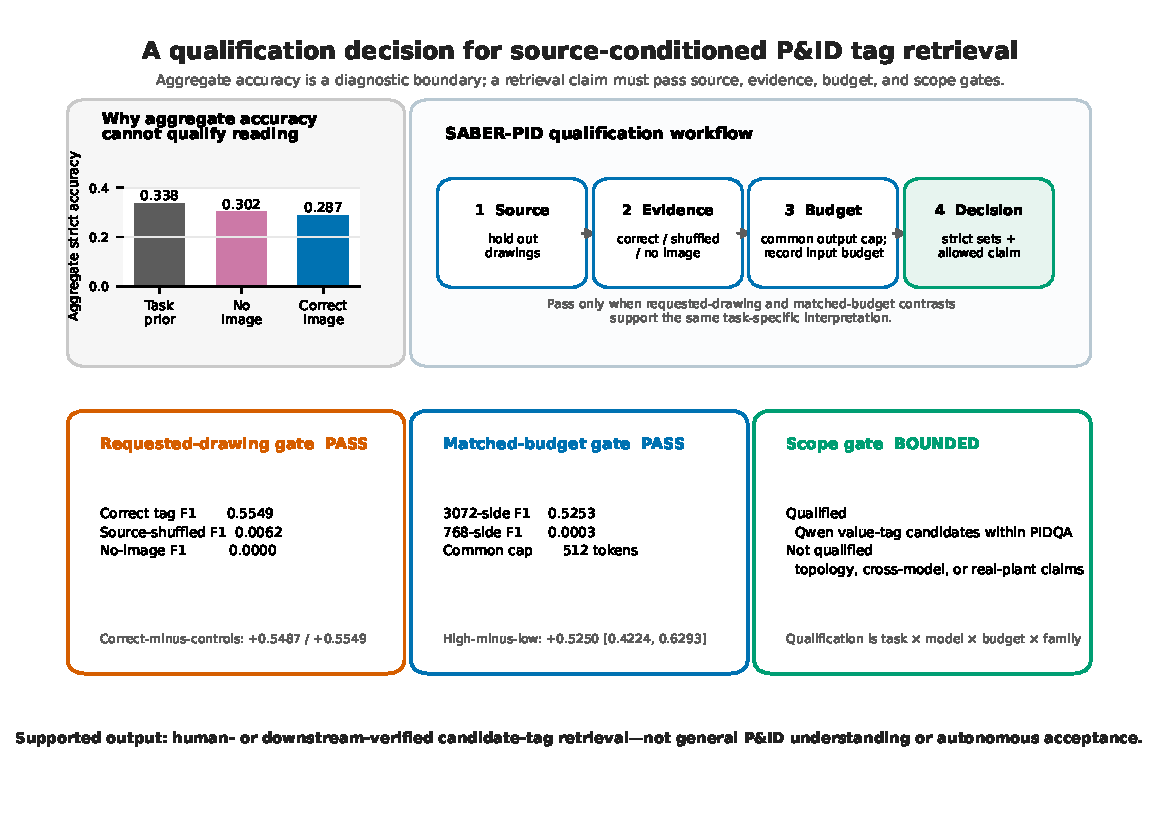
\includegraphics[width=\linewidth]{figure_1_qualification_decision_v6.pdf}
\caption{Qualification decision. Aggregate accuracy is retained as a
diagnostic boundary. A task-specific claim proceeds through source,
counterfactual-evidence, matched-budget, and scope gates. Values are generated
from the frozen analysis artifacts.}
\label{fig:decision}
\end{figure}

Across the five split seeds, the input-retrieval-plus-prior diagnostic scores
50.9\% under question-random splitting and 31.5\% under source isolation, a
mean difference of 19.5 percentage points (individual differences 13.6--21.3
points). Exact-image semantic-cache hits create the additional route only
when the same drawing crosses the split. The result motivates drawing-level
isolation without claiming that the evaluated VLM used that route.

\subsection{The tag signal follows the requested drawing and visual-input budget}

At 3072-side and 192 output tokens, Qwen produces 192 true positives, 152 false
positives, and 156 false negatives. Pooled precision, recall, F1, and exact-set
accuracy are 0.5581, 0.5517, 0.5549, and 0.1900. Source-macro F1 is 0.5810
([0.5118, 0.6501]); excluding the seven empty-reference sources gives 0.6139.
Correct minus source-shuffled pooled F1 is +0.5487 ([0.4729, 0.6239]), and
correct minus no-image is +0.5549 ([0.4799, 0.6322]). Thus, the useful signal
tracks the requested source drawing rather than the prompt or arbitrary
P\&ID pixels.

At a common 512-token cap, the high-minus-low visual-input-budget effect is
+0.5250 ([0.4224, 0.6293]). At the original 192-token cap it is +0.5549
([0.4774, 0.6314]). The seed-29 and seed-31 descriptive partitions yield
+0.6783 ([0.6163, 0.7384]) and +0.6500 ([0.5684, 0.7295]). All four effects
are positive, while only Set B carries the primary qualification role.

\begin{figure}[!htbp]
\centering
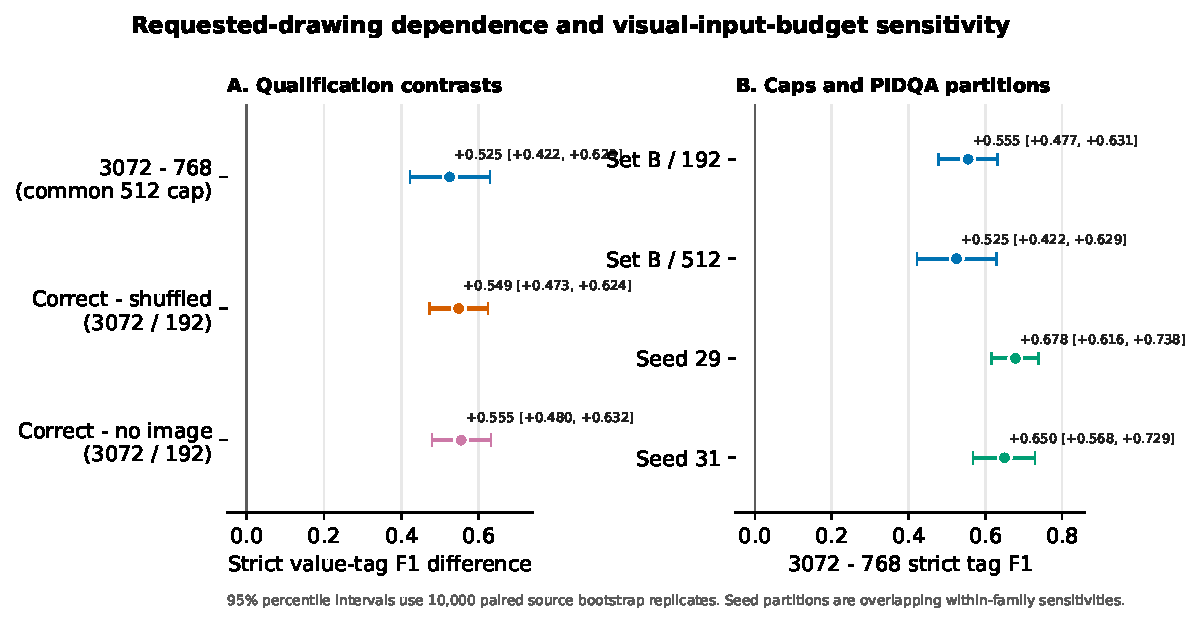
\includegraphics[width=\linewidth]{figure_2_qualification_effects_v6.pdf}
\caption{Paired task-specific qualification effects. Panel A contrasts
correctly paired, source-shuffled, and absent image evidence. Panel B compares
visual-input budgets under two output caps and two descriptive source
partitions. Intervals use 10,000 paired source-cluster bootstrap replicates.}
\label{fig:effects}
\end{figure}

\subsection{The requested-drawing effect replicates across scales, prompts, and subsets}

The frozen extension contains 36 correct-minus-control comparisons. All 36
source-bootstrap intervals have positive lower bounds. Across the six
subset--prompt cells, Qwen3-VL-8B correct-image value-tag F1 ranges from
0.5253 to 0.6587 (median 0.6229); correct-minus-shuffled effects range from
+0.5191 to +0.6437, and correct-minus-no-image effects from +0.5253 to
+0.6587. Qwen3-VL-32B correct-image F1 ranges from 0.5697 to 0.7361 (median
0.6512); its corresponding effect ranges are +0.5639--+0.7284 and
+0.5697--+0.7361. Thus, the requested-drawing signal is not confined to one
Qwen scale, subset, or wording.

InternVL3.5-8B also has positive correct-minus-control intervals in all 12
comparisons, but correct-image F1 remains 0.0090--0.0257 (median 0.0124).
The direction therefore transfers more broadly than the useful magnitude.
Eight of nine P1-minus-P0 intervals include zero; the exception is a small
negative effect for Qwen3-VL-32B on seed 29. Figure~\ref{fig:v7replication}
reports every pre-specified contrast rather than selecting a prompt or subset.

\begin{figure}[!htbp]
\centering
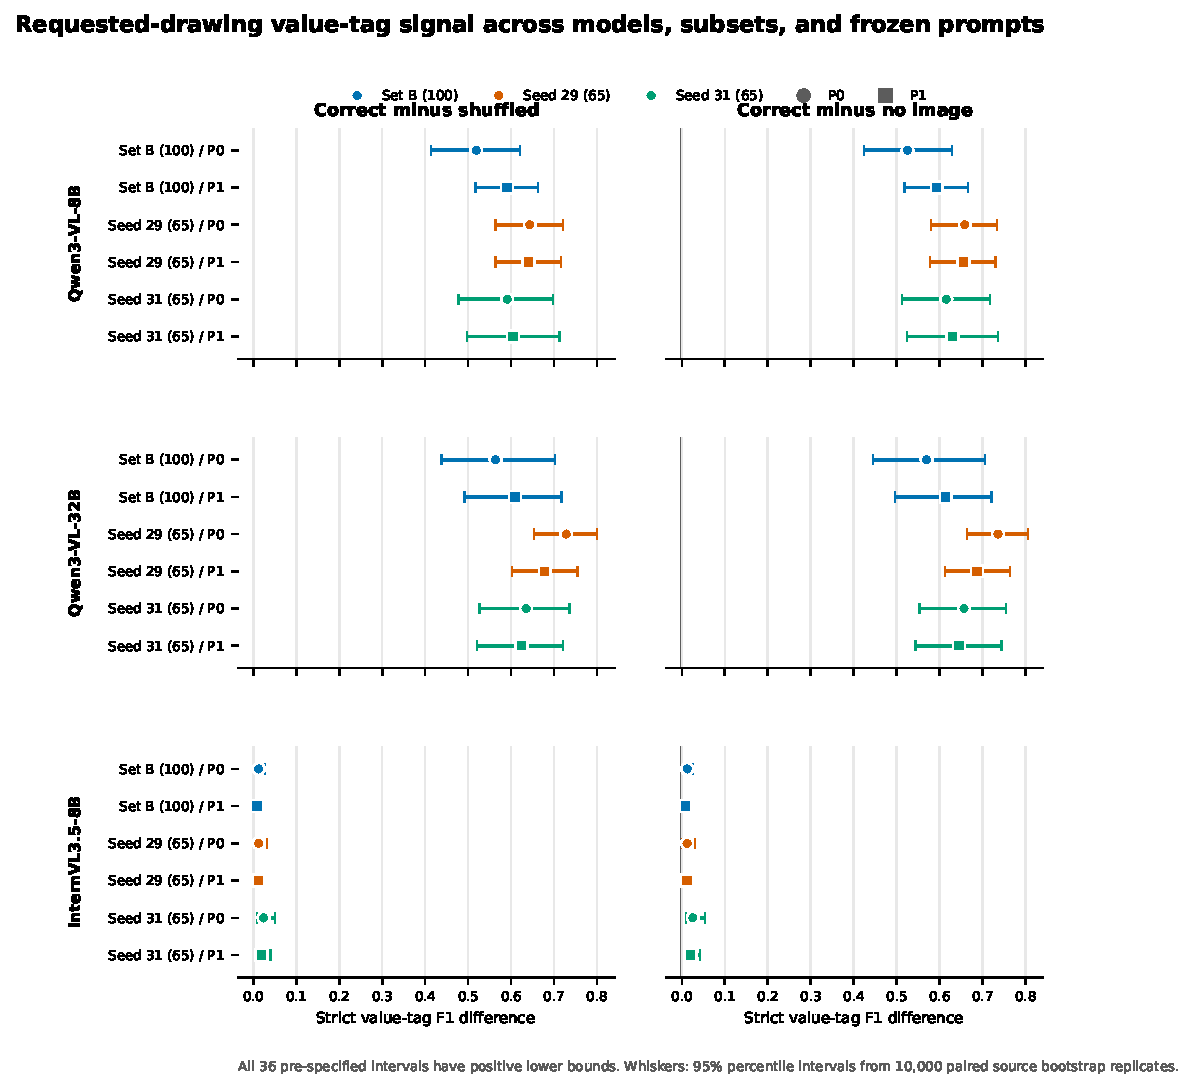
\includegraphics[width=\linewidth]{figure_v7_cross_model_counterfactual_replication.pdf}
\caption{Frozen cross-model counterfactual replication. Rows cross three
models with three pairwise source-disjoint PIDQA subsets and two pre-existing
prompts. Columns show correct-image minus source-shuffled and correct-image
minus no-image strict value-tag F1. Whiskers are 95\% percentile intervals
from 10,000 paired source bootstrap replicates.}
\label{fig:v7replication}
\end{figure}

\subsection{OCR and VLM outputs support distinct operating modes}

Table~\ref{tab:operating} reports counts and both F1 estimators. Geometry-
joined OCR has fewer false positives than Qwen and pooled F1 0.5933. Union
recovers 245 of 348 reference tags, increasing recall to 0.7040 and pooled F1
to 0.6339. Its pooled union-minus-Qwen difference is +0.0790
([0.0372, 0.1261]); the source-macro difference is +0.0792
([0.0373, 0.1250]). Non-empty-reference source-macro F1 is 0.6991 for union
and 0.6139 for Qwen.

Intersection produces only one false candidate among 107 candidates:
precision 0.9907 with source-bootstrap interval [0.9681, 1.0000], at recall
0.3046. OCR-first fallback reaches pooled F1 0.6228 and exact-set accuracy
0.2200. These are transparent retrieval modes, not a learned ensemble.

\begin{table}[!htbp]
\centering
\caption{Set B candidate-tag performance on 100 sources. Micro values pool
TP/FP/FN; macro F1 weights each source equally.}
\label{tab:operating}
\scriptsize
\resizebox{\linewidth}{!}{%
\begin{tabular}{lrrrrrrrr}
\toprule
Mode & TP & FP & FN & Precision & Recall & Micro F1 & Macro F1 & Exact \\
\midrule
Qwen, correct image, 3072/192 & 192 & 152 & 156 & 0.5581 & 0.5517 & 0.5549 & 0.5810 & 0.1900 \\
OCR, literal parse & 116 & 44 & 232 & 0.7250 & 0.3333 & 0.4567 & 0.4227 & 0.1200 \\
OCR, geometry join & 159 & 29 & 189 & 0.8457 & 0.4569 & 0.5933 & 0.5618 & 0.2100 \\
Set union & 245 & 180 & 103 & 0.5765 & 0.7040 & 0.6339 & 0.6602 & 0.1900 \\
Set intersection & 106 & 1 & 242 & 0.9907 & 0.3046 & 0.4659 & 0.4312 & 0.1700 \\
OCR if non-empty, else Qwen & 175 & 39 & 173 & 0.8178 & 0.5029 & 0.6228 & 0.6073 & 0.2200 \\
\bottomrule
\end{tabular}}
\end{table}

The median candidates per drawing [IQR] are 3 [1, 4] for Qwen, 2 [1, 3] for
joined OCR, 4 [2, 5] for union, 1 [0, 2] for intersection, and 2 [1, 3] for
OCR-first fallback. Median false candidates are respectively 0 [0, 2],
0 [0, 0], 1 [0, 2], 0 [0, 0], and 0 [0, 1]. Intersection is empty on 41
drawings, while union, Qwen, and OCR-first are empty on one each. This
quantifies the coverage--review-burden trade-off behind Figure~\ref{fig:modes}.

\begin{figure}[!htbp]
\centering
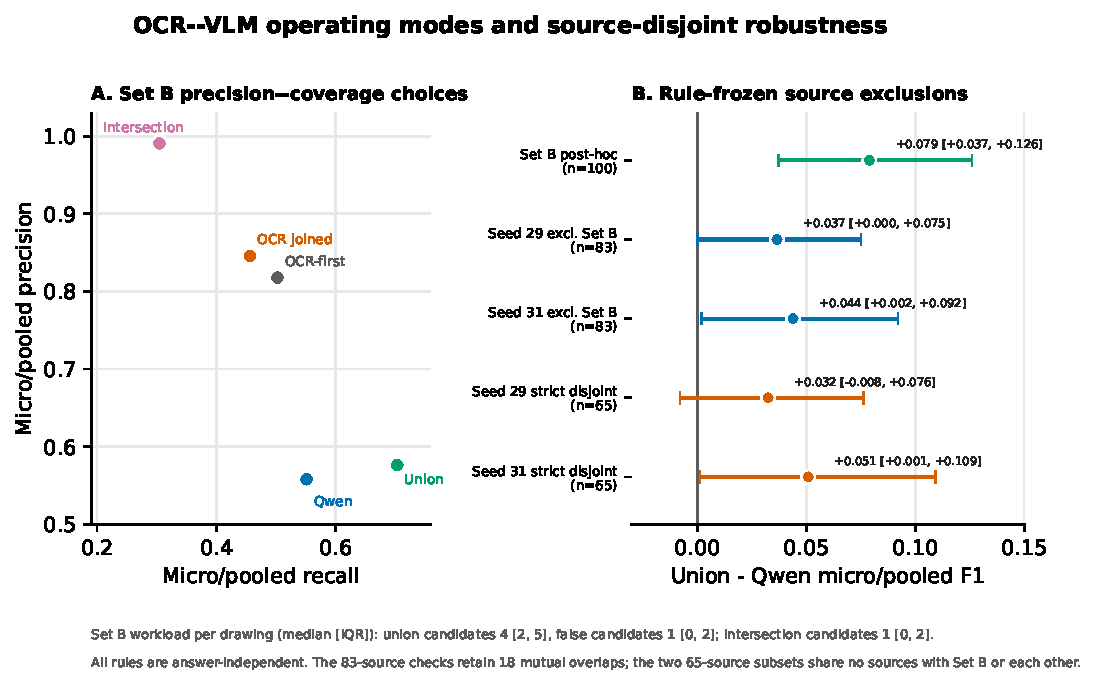
\includegraphics[width=\linewidth]{figure_3_operating_modes_v6.pdf}
\caption{Reference-free operating modes and overlap-audited stability checks.
Panel A gives Set B precision--recall locations. Panel B shows pooled
union-minus-Qwen F1 for Set B, Set-B-excluded 83-source subsets, and mutually
disjoint 65-source subsets. The footer reports per-drawing candidate workload.}
\label{fig:modes}
\end{figure}

\subsection{Cost-sensitive loss yields an explicit operating-mode rule}

The observed count vectors turn the coverage--precision choices into four
loss lines: intersection $242r+1$, joined OCR $189r+29$, OCR-first
$173r+39$, and union $103r+180$. Their exact lower envelope selects
intersection for $r<0.5283$, joined OCR for $0.5283<r<0.6250$, OCR-first for
$0.6250<r<2.0143$, and union for $r>2.0143$; adjacent modes tie at each
boundary. Thus a workflow in which a missed tag costs roughly the same as a
false candidate selects OCR-first, while sufficiently miss-sensitive use
selects union and sufficiently review-sensitive use selects intersection.

Source resampling shows that uncertainty is concentrated near the switches,
not at the low- and high-cost extremes. The descriptive pairwise switch-ratio
medians [95\% intervals] are 0.532 [0.293, 0.958], 0.611 [0.176, 1.750], and
2.000 [1.200, 3.323]. Joined OCR occupies a narrow point-estimate interval and
has a maximum minimum-loss bootstrap probability of 0.347, whereas OCR-first
reaches 0.889 near $r=1.25$. Figure~\ref{fig:costdecision} therefore reports
both the exact count-based rule and its source-bootstrap decision stability.

\begin{figure}[!htbp]
\centering
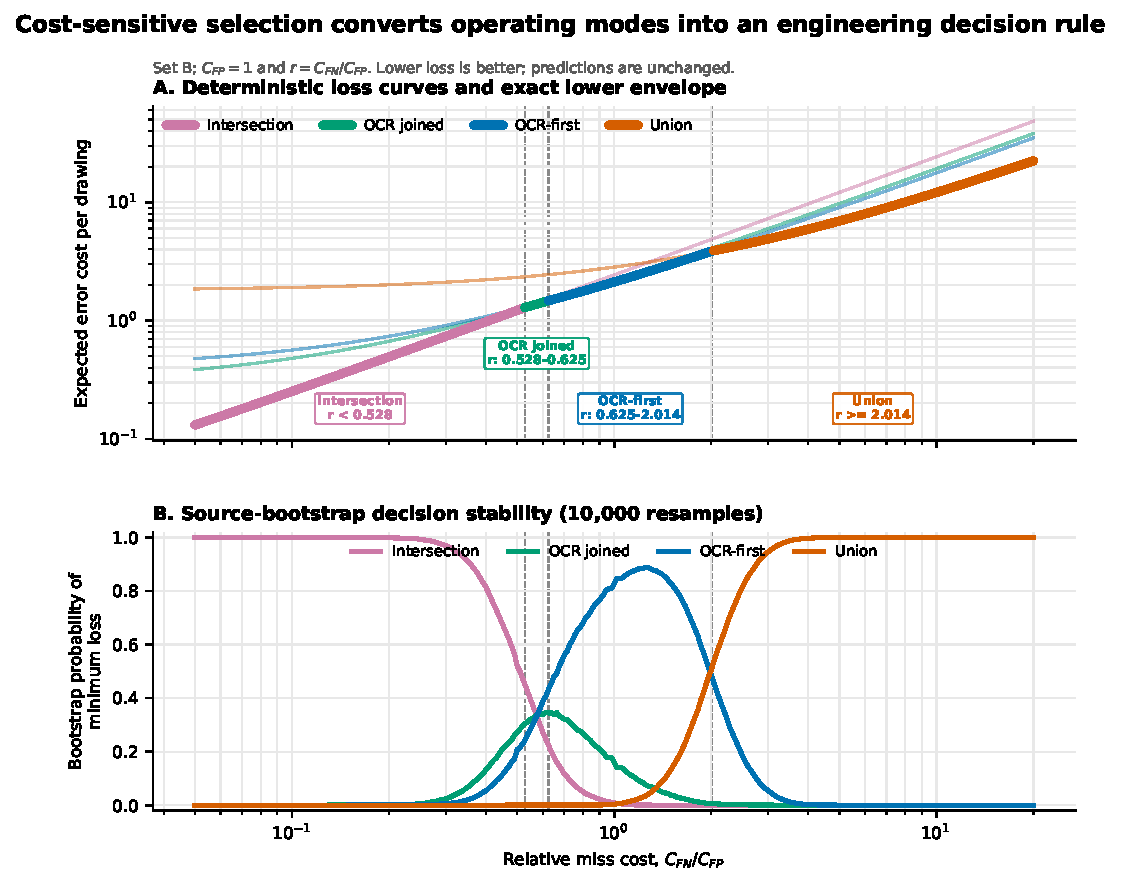
\includegraphics[width=\linewidth]{figure_4_cost_sensitive_operating_modes_v8.pdf}
\caption{Cost-sensitive operating-mode decision. Panel A plots normalized
Set B loss $L=rFN+FP$ per drawing and highlights the exact lower envelope.
Panel B shows each mode's probability of minimum loss over 10,000
source-cluster resamples. Dashed lines mark the three point-estimate switches;
predictions are unchanged by this scorer-only analysis.}
\label{fig:costdecision}
\end{figure}

\subsection{Mild image-quality shifts preserve requested-drawing evidence at the qualified budget}

The paired robustness matrix holds the qualified Qwen input and output budgets
at 3072-side/512 tokens and pools three mutually source-disjoint subsets (230
drawings; 7,360 predictions). Correct-image strict tag F1 is 0.5693 on clean
images, 0.5836 after JPEG quality 70, 0.5879 after Gaussian blur radius 1, and
0.5605 after 0.75$\times$ downsample-and-restore. The corresponding shuffled-
image F1 values are 0.0114, 0.0114, 0.0125, and 0.0123. Correct-minus-shuffled
effects are therefore +0.5578 ([0.4917, 0.6227]), +0.5722 ([0.5060, 0.6344]),
+0.5754 ([0.5101, 0.6356]), and +0.5482 ([0.4763, 0.6134]), respectively.

The paired change in this counterfactual effect relative to clean is +0.0143
([-0.0034, 0.0345]) for JPEG, +0.0176 ([-0.0155, 0.0517]) for blur, and
-0.0096 ([-0.0655, 0.0520]) for downsample-and-restore. Every interval includes
zero. Thus the declared mild shifts retain a large requested-drawing effect and
show no detected deterioration relative to clean; this result does not qualify
more severe scanning, occlusion, or revision-mark conditions.

\begin{table}[H]
\centering
\caption{Paired quality robustness at the qualified Qwen 3072-side/512-token setting, pooled over 230 pairwise source-disjoint drawings. Intervals use 10,000 paired source-bootstrap replicates. The final column is the change in the correct-minus-shuffled effect relative to clean.}
\label{tab:v8quality}
\scriptsize
\resizebox{\linewidth}{!}{%
\begin{tabular}{lrrrr}
\toprule
Condition & Correct F1 & Shuffled F1 & Correct$-$shuffled [95\% interval] & Change vs clean [95\% interval] \\
\midrule
Clean & 0.5693 & 0.0114 & +0.5578 [+0.4917, +0.6227] & -- \\
JPEG Q70 & 0.5836 & 0.0114 & +0.5722 [+0.5060, +0.6344] & +0.0143 [-0.0034, +0.0345] \\
Blur $r=1$ & 0.5879 & 0.0125 & +0.5754 [+0.5101, +0.6356] & +0.0176 [-0.0155, +0.0517] \\
0.75$\times$ restore & 0.5605 & 0.0123 & +0.5482 [+0.4763, +0.6134] & -0.0096 [-0.0655, +0.0520] \\
\bottomrule
\end{tabular}}
\end{table}


\subsection{A closer visual budget recovers strong InternVL requested-drawing dependence}

The closest-safe InternVL matrix contains nine complete cells and 2,760
predictions. Pooled over the same 230 mutually source-disjoint drawings,
correct-image strict tag F1 is 0.4846, compared with 0.0131 under source
shuffling and 0 without an image. The correct-minus-shuffled effect is +0.4715
([0.4064, 0.5332]); the correct-minus-no-image effect is +0.4846 ([0.4198,
0.5463]). Every subset-specific correct-minus-control interval has a positive
lower bound.

Relative to the earlier native-12-tile correct-image cells, the pooled 54-tile
gain is +0.4681 ([0.4043, 0.5290]); subset gains are +0.4458--+0.4964, all with
positive lower bounds. The 54-tile tensor contains 9.63\% fewer recorded input
elements than the qualified Qwen processor, so this is not encoder equivalence.
It does show that visual-budget adequacy is a first-class qualification
variable and that requested-drawing dependence transfers to a second model
family when gross input-budget mismatch is reduced.

\begin{figure}[!htbp]
\centering
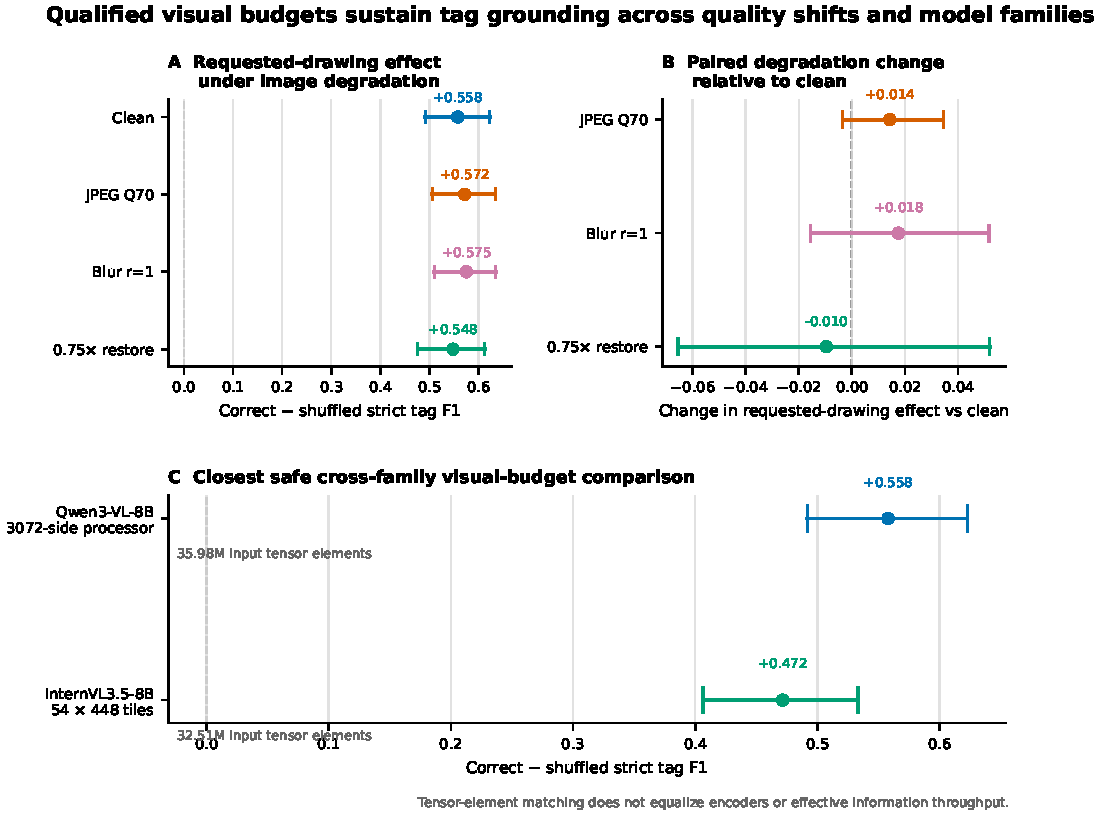
\includegraphics[width=\linewidth]{figure_5_quality_and_budget_matched_v8.pdf}
\caption{Qualified-budget robustness and cross-model visual-budget recovery.
Panel A reports correct-minus-shuffled strict tag F1 under clean and three mild
quality shifts. Panel B reports the paired change in that effect relative to
clean. Panel C shows the large requested-drawing effect recovered by the
54-tile InternVL input at the closest safe recorded tensor-element budget.
Intervals use 10,000 paired source-
bootstrap replicates; tensor-element matching does not equalize encoders.}
\label{fig:v8quality}
\end{figure}

\subsection{A second public P\&ID family transfers the qualification}

The visibility-qualified DEXPI branch supplies 65 prefix-conditioned tag
questions from 35 images in 26 logical test cases. On the exact image/XML
pairs, Qwen produces 72 true positives, six false positives, and nine false
negatives: precision 0.9231, recall 0.8889, strict tag F1 0.9057, exact-set
accuracy 0.8615, and logical-case-macro exact accuracy 0.9006. Cross-case
shuffling produces zero true positives, 144 false positives, and F1 0; the
no-image condition also has F1 0. Correct-minus-shuffled and correct-minus-no-
image effects are both +0.9057, with case-bootstrap intervals [0.8409, 0.9841]
and [0.8431, 0.9844].

The frozen full-image OCR comparator reaches precision 0.9608, recall 0.6049,
F1 0.7424, and exact-set accuracy 0.6154. Qwen correct-image minus OCR F1 is
+0.1632 ([0.0317, 0.3882]); OCR minus no-image is +0.7424 ([0.5435, 0.8504]).
The family, visibility rule, image/XML pairing, and derangement were selected
without model outputs. This is strong transfer evidence to a second public
drawing family, while its size and training-example style still do not
establish real-plant deployment performance.

\begin{table}[H]
\centering
\caption{External-family tag retrieval on 65 questions from 35 DEXPI images in 26 logical test cases. Vendor variants are grouped by logical case for uncertainty estimates.}
\label{tab:v8dexpi}
\scriptsize
\resizebox{\linewidth}{!}{%
\begin{tabular}{lrrrrrrr}
\toprule
Condition & TP & FP & FN & Precision & Recall & F1 & Exact \\
\midrule
Qwen, correct image & 72 & 6 & 9 & 0.9231 & 0.8889 & 0.9057 & 0.8615 \\
Qwen, cross-case shuffled & 0 & 144 & 81 & 0.0000 & 0.0000 & 0.0000 & 0.0000 \\
Qwen, no image & 0 & 0 & 81 & 1.0000 & 0.0000 & 0.0000 & 0.0000 \\
PaddleOCR, full image & 49 & 2 & 32 & 0.9608 & 0.6049 & 0.7424 & 0.6154 \\
\bottomrule
\end{tabular}}
\end{table}


\begin{figure}[!htbp]
\centering
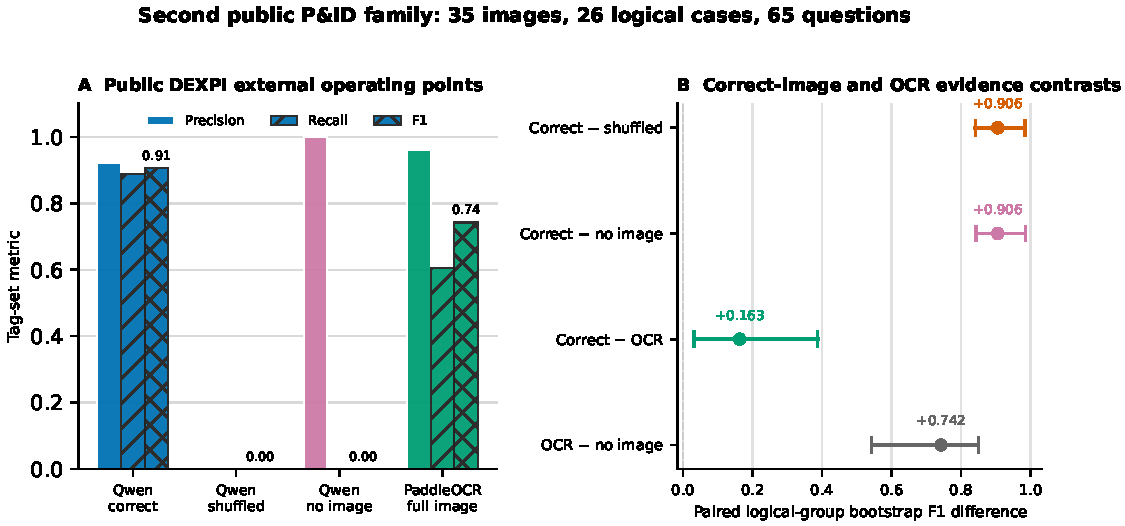
\includegraphics[width=\linewidth]{figure_6_dexpi_external_v8.pdf}
\caption{External-family tag retrieval on public DEXPI drawings. Panel A shows
precision, recall, and F1 for Qwen correct, cross-case shuffled, no-image, and
full-image OCR conditions. Panel B gives logical-case-bootstrap F1 contrasts.
All 65 predictions per condition are retained; no result-guided source or tag
selection is applied.}
\label{fig:v8dexpi}
\end{figure}

\subsection{Geometry joining and error complementarity explain the operating envelope}

The reference-free OCR geometry rule performs 45 prefix--suffix joins. Relative
to literal parsing, it adds 44 true tags and one false candidate while removing
16 false candidates and one true tag. Per-source F1 improves on 16 drawings,
degrades on one, and is unchanged on 83. Pooled F1 increases from 0.4567 to
0.5933. This ablation supports the deterministic join as an engineering text
normalization step rather than a reference-aware correction.

Of 348 true tags, 106 are recovered by both instruments, 86 only by Qwen, 53
only by OCR, and 103 by neither. Of 180 distinct false candidates appearing in
their union, only one appears in both; 151 are Qwen-only and 28 OCR-only. At
source level, Qwen contributes a unique true tag on 43 drawings, OCR on 17,
and both contribute unique true tags on seven. The deterministic error
taxonomy further shows that Qwen has 19 exact-set sources and 38 partial-
recovery sources with false candidates, whereas joined OCR has 21 exact-set
sources, 15 partial-recovery sources with false candidates, and 12 empty
predictions against non-empty references. The full taxonomy and string-form
diagnostics are reported in the supplement without causal interpretation.

\subsection{Overlap-audited frozen-rule checks retain the direction with asymmetric strength}

Set B overlaps seed 29 and seed 31 by 17 sources each; seed 29 and seed 31
overlap each other by 20 sources, including two shared by all three sets.
Removing Set B leaves 83 sources per partition, with 18 still shared between
the two partitions. On these Set-B-excluded subsets, pooled union-minus-Qwen
F1 is +0.0366 ([0.0002, 0.0751]) and +0.0440 ([0.0021, 0.0920]).
Source-macro effects are +0.0451 ([0.0043, 0.0892]) and +0.0373
([-0.0082, 0.0854]).

Removing the residual cross-partition overlap yields 65 sources per strict
subset. Pooled differences are +0.0325 ([-0.0078, 0.0764]) and +0.0509
([0.0012, 0.1093]); source-macro differences are +0.0379
([-0.0088, 0.0885]) and +0.0425 ([-0.0123, 0.0974]). The direction is positive
in every point estimate, but interval exclusion of zero depends on subset and
estimator. This supports a cautious within-family stability statement, not an
independent-replication claim.

\begin{table}[!htbp]
\centering
\caption{Frozen union rule after source-overlap exclusions. Intervals are
paired 95\% source-bootstrap intervals.}
\label{tab:transfer}
\small
\begin{tabular}{lrrrr}
\toprule
Subset & $n$ & Qwen micro F1 & Union micro F1 & Difference [95\% interval] \\
\midrule
Seed 29 excluding Set B & 83 & 0.6717 & 0.7083 & +0.0366 [0.0002, 0.0751] \\
Seed 31 excluding Set B & 83 & 0.6417 & 0.6856 & +0.0440 [0.0021, 0.0920] \\
Seed 29 strictly disjoint & 65 & 0.6587 & 0.6911 & +0.0325 [-0.0078, 0.0764] \\
Seed 31 strictly disjoint & 65 & 0.6158 & 0.6667 & +0.0509 [0.0012, 0.1093] \\
\bottomrule
\end{tabular}
\end{table}

\subsection{Boundary analyses delimit the supported claim}

The qualification does not extend to topology or arbitrary model families.
At the same 3072/192 Qwen operating point, correct-image aggregate strict
accuracy is 0.2875 and no-image accuracy is 0.3025 because structural tasks
retain strong prior pathways. A visible symbol legend changes spatial-count
accuracy, but correct numeric labels show no detected advantage over a
layout-matched label permutation (interval [-0.04, 0.04]). The initial
corrected InternVL3.5-8B check produces correct-image tag F1 0.0126 and zero
under source-shuffled and no-image conditions. The larger frozen native-budget
matrix confirms the direction but bounds correct-image F1 at 0.0090--0.0257.
In contrast, the closest-safe 54-tile input reaches pooled F1 0.4846 and a
+0.4715 correct-minus-shuffled effect. The +0.4681 paired gain over native 12
tiles identifies visual budget as the operative boundary rather than model
identity alone. Because tensor-element matching does not equalize encoders,
these results still do not support a universal visual-input law, topology
reasoning, or cross-model performance equivalence.

\section{Discussion}

\subsection{Engineering interpretation}

The principal result is a bounded qualification: high-detail Qwen inference
provides image-grounded candidate-tag retrieval on unseen PIDQA drawings.
Correct/source-shuffled/no-image interventions localize the signal to the
requested drawing, and the matched-output-cap comparison shows that the
effect is not explained by a larger text-generation allowance. The aggregate
score would have obscured this capability because nonvisual pathways dominate
other task families. Reporting by task is therefore not merely presentational;
it changes the engineering decision.

Three extensions strengthen that localization without broadening it beyond the
measured task. At the same qualified 3072/512 budget, three mild image-quality
changes preserve large correct-minus-shuffled effects and show no detected
change from clean. Reducing the gross visual-budget mismatch raises pooled
InternVL correct-image F1 from the native-budget range to 0.4846 and yields a
+0.4715 requested-drawing effect, providing a cross-family replication at a
declared closest-safe input budget. On a separately licensed public DEXPI family, exact image/
XML pairing yields F1 0.9057 while cross-case shuffled and no-image controls
yield zero. The latter is an external-family transfer result rather than a
second partition of PIDQA, although 35 images in curated training examples do
not represent the diversity of operating-plant documents.

The OCR--VLM operating envelope turns the qualification into selectable
workflow modes. Union emphasizes coverage (recall 0.7040) at a median of four
candidates and one false candidate per drawing. Intersection yields an
approximately one-candidate conservative shortlist with precision 0.9907 but
is empty on 41\% of drawings. OCR-first fallback provides a middle operating
point with pooled F1 0.6228, a median of two candidates, and median zero false
candidates. The cost rule makes that choice executable: use intersection when
$C_{FN}/C_{FP}<0.528$, joined OCR in the narrow 0.528--0.625 interval,
OCR-first from 0.625--2.014, and union above 2.014, while treating the
bootstrap panel as uncertainty around a Set-B-derived rule rather than a
universal tariff.

\subsection{Why the evaluation contract matters}

SABER-PID joins four controls that are often considered separately.
Drawing-level splitting removes an input-recoverable same-source route.
Answer-hidden manifests separate inference from scoring. Counterfactual
images test source identity and image presence directly. Recorded visual and
output budgets make the high--low comparison interpretable. Finally, pooled
and source-macro estimates show that conclusions are not an artifact of
drawings with many tags.

The phase distinction is equally important. The Set B fusion result is a
descriptive analysis formed after component inspection. Later rule checks
freeze all operations, but their shared PIDQA family and source overlaps limit
their evidential role. Explicit exclusions reveal the honest result: the
positive direction persists, while uncertainty is sensitive to subset size
and estimator. This is stronger and more useful than either suppressing the
overlap or overstating the checks as independent evidence.

\subsection{Implications for engineering document intelligence}

The evaluated output is a candidate set for indexing or subsequent
deterministic validation, not an autonomous engineering decision. This
distinction aligns with practical P\&ID digitization: text recognition is one
layer of a larger pipeline that may incorporate format rules, master-data
matching, and topology checks \cite{kim2021,shteriyanov2026}. The present
results show when the image supplies usable tag evidence and how two frozen
instruments trade coverage for precision. They do not remove the need for
project-specific identifier rules or validation against controlled
engineering data.

\section{Limitations}

The primary operating-mode and robustness analyses use the public synthetic
500-sheet PIDQA family. Source isolation protects unseen-sheet evaluation
within that family but does not establish performance on scanned, revision-
marked, proprietary, or project-specific plant drawings. DEXPI adds a second
licensed public family, but the evaluated scope is only 35 visibility-qualified
images from curated training examples and 65 tag questions; it is not a field
sample. The primary operating point concerns one frozen Qwen3-VL-8B prompt and
decoding configuration. The extension covers two frozen prompts and a 32B
Qwen scale. The large change from native-12 to 54-tile InternVL shows that
performance is not visual-budget-invariant; matching recorded tensor elements
still does not equalize architectures, encoders, or effective information
throughput. Only one non-Qwen checkpoint was evaluated. The OCR comparator is a frozen full-image pipeline rather
than an optimized industrial recognizer.

Set B fusion is descriptive. Frozen-rule checks remain within PIDQA, and even
after Set B exclusion the two 83-source subsets share sources; the stricter
65-source results have wider intervals. The 100-source controls estimate
discrete operating points, not a continuous or universal visual-input law.
The quality matrix covers three declared mild transformations at one severity
each; it does not support robustness claims for heavy compression, severe
blur, occlusion, handwriting, or arbitrary scan pipelines.
Latency co-varies with generated output length and is not interpreted as pure
image-encoding cost. Candidate workload is computed against benchmark
references; field verification effort may differ.

PID2Graph/OPEN100 was also screened as a possible second tag-retrieval family
\cite{stuermer2025}.
An HTTP byte-range audit read the official ZIP catalogue and materialized all
24 image/GraphML members for 12 complete plans without downloading the full
9.3-GB archive. The GraphML supplies structural node classes, edge classes,
and bounding boxes, but no explicitly named text, tag, or identifier field;
internal node IDs were not treated as visible drawing strings. PID2Graph is
therefore retained as a structural-data resource and not assigned a tag-
retrieval score. The external tag experiment instead uses the visibility-
qualified DEXPI pairs described above.

\section{Conclusion}

Candidate-tag retrieval from P\&IDs can be qualified only when the evidence is
reported at the task, source, model, and budget levels. On source-isolated
PIDQA drawings, high-detail Qwen inference passes requested-drawing and
matched-budget gates: pooled F1 is 0.5549 with the correct image, 0.0062 with a
source-shuffled image, and zero without an image. A 54-cell frozen extension
retains positive requested-drawing intervals in all 36 contrasts across two
Qwen scales, InternVL, two prompts, and three source-disjoint subsets. A
separate closest-safe 54-tile pass then raises pooled InternVL correct-image F1
to 0.4846 and its correct-minus-shuffled effect to +0.4715, demonstrating
cross-model transfer after visual-budget qualification. OCR and Qwen recover
complementary tags. Reference-free union reaches recall 0.7040 and pooled F1
0.6339, while intersection reaches precision 0.9907; the cost-sensitive rule
makes their selection explicit. Mild JPEG, blur, and resampling changes retain
large requested-drawing effects at the qualified budget. On 35 public DEXPI
images, correct-image Qwen reaches F1 0.9057 while shuffled and no-image
controls remain at zero. Overlap-audited frozen-rule checks preserve positive
point estimates but also expose estimator- and subset-dependent uncertainty.
The resulting conclusion is deliberately bounded: SABER-PID supports
configurable candidate-tag retrieval under the evaluated PIDQA and DEXPI
conditions; it does not qualify topology reasoning, general P\&ID
understanding, or field deployment.

\section*{Data and code availability}

The submission package contains a locally validated reproducibility archive
with answer-isolated public manifests, scorer-only references, immutable raw
generation JSONL, deterministic analysis and figure scripts, tests,
environment records, and SHA-256 manifests. PIDQA/Dataset-PID source data are
covered by the vendored CC0 record; complete image collections are acquired by
reference, and model weights are not redistributed. The submitter must upload
this archive to a public repository and replace
\texttt{[SUBMITTER: ARCHIVE DOI/URL]} before submission.

\section*{Declaration of competing interest}
The submitting authors must insert and approve the applicable competing-
interest declaration before upload; no declaration is inferred by the
automated revision workflow.

\section*{Funding}
The submitting authors must insert the applicable funding statement before
upload.

\section*{Use of generative AI and AI-assisted technologies}
OpenAI Codex was used to assist analysis-code development, deterministic
validation, figure generation, and manuscript editing. ChatGPT Pro was used
for an author-side model-based editorial critique. All numerical statements
in the manuscript were regenerated from machine-readable artifacts, and all
figures were rendered by deterministic plotting code rather than a generative
image model. The authors remain responsible for verification and the final
submitted text.

\begin{thebibliography}{99}
\raggedright
\bibitem{rahul2019} R. Rahul, S. Paliwal, M. Sharma, and L. Vig, \emph{Automatic information extraction from piping and instrumentation diagrams}, arXiv:1901.11383, 2019.
\bibitem{paliwal2021} S. Paliwal, A. Jain, M. Sharma, and L. Vig, \emph{Digitize-PID: Automatic digitization of piping and instrumentation diagrams}, arXiv:2109.03794, 2021.
\bibitem{kim2021} H. Kim, W. Lee, M. Kim, Y. Moon, T. Lee, M. Cho, and D. Mun, \emph{Deep-learning-based recognition of symbols and texts at an industrially applicable level from images of high-density piping and instrumentation diagrams}, Expert Systems with Applications 183 (2021) 115337. doi:10.1016/j.eswa.2021.115337.
\bibitem{su2024} G. Su, S. Zhao, T. Li, S. Liu, Y. Li, G. Zhao, and Z. Li, \emph{Image format pipeline and instrument diagram recognition method based on deep learning}, Biomimetic Intelligence and Robotics 4(1) (2024) 100142. doi:10.1016/j.birob.2023.100142.
\bibitem{shteriyanov2026} V. Shteriyanov, R. Dzhusupova, J. Bosch, and H. Holmstr\"om Olsson, \emph{From text to meaning: Semantic interpretation of non-standardized metadata in piping and instrumentation diagrams}, Computers \& Chemical Engineering 204 (2026) 109436. doi:10.1016/j.compchemeng.2025.109436.
\bibitem{gupta2025} M. Gupta, C. Wei, T. Czerniawski, and R. Eiris, \emph{PIDQA---Question answering on piping and instrumentation diagrams}, Machine Learning and Knowledge Extraction 7(2) (2025) 39. doi:10.3390/make7020039.
\bibitem{geras2013} K. Geras and C. Sutton, \emph{Multiple-source cross-validation}, Proceedings of the 30th International Conference on Machine Learning, PMLR 28(3) (2013) 1292--1300.
\bibitem{kapoor2023} S. Kapoor and A. Narayanan, \emph{Leakage and the reproducibility crisis in machine-learning-based science}, Patterns 4 (2023) 100804. doi:10.1016/j.patter.2023.100804.
\bibitem{mathew2021} M. Mathew, D. Karatzas, and C. V. Jawahar, \emph{DocVQA: A dataset for VQA on document images}, Proceedings of WACV (2021) 2200--2209.
\bibitem{masry2022} A. Masry, D. X. Long, J. Q. Tan, S. Joty, and E. Hoque, \emph{ChartQA: A benchmark for question answering about charts with visual and logical reasoning}, Findings of ACL (2022) 2263--2279. doi:10.18653/v1/2022.findings-acl.177.
\bibitem{nourbakhsh2025} A. Nourbakhsh, S. Parekh, P. Shetty, Z. Jin, S. Shah, and C. Rose, \emph{Where is this coming from? Making groundedness count in the evaluation of Document VQA models}, Findings of NAACL (2025) 5341--5361. doi:10.18653/v1/2025.findings-naacl.295.
\bibitem{chen2020} L. Chen, X. Yan, J. Xiao, H. Zhang, S. Pu, and Y. Zhuang, \emph{Counterfactual samples synthesizing for robust visual question answering}, Proceedings of CVPR (2020) 10800--10809. doi:10.1109/CVPR42600.2020.01081.
\bibitem{li2023pope} Y. Li, Y. Du, K. Zhou, J. Wang, X. Zhao, and J.-R. Wen, \emph{Evaluating object hallucination in large vision-language models}, Proceedings of EMNLP (2023) 292--305. \url{https://doi.org/10.18653/v1/2023.emnlp-main.20}.
\bibitem{leng2024} S. Leng, H. Zhang, G. Chen, X. Li, S. Lu, C. Miao, and L. Bing, \emph{Mitigating object hallucinations in large vision-language models through visual contrastive decoding}, Proceedings of CVPR (2024) 13872--13882.
\bibitem{du2020} Y. Du et al., \emph{PP-OCR: A practical ultra lightweight OCR system}, arXiv:2009.09941, 2020.
\bibitem{bai2025} S. Bai et al., \emph{Qwen3-VL technical report}, arXiv:2511.21631, 2025.
\bibitem{wang2025} W. Wang et al., \emph{InternVL3.5: Advancing open-source multimodal models in versatility, reasoning, and efficiency}, arXiv:2508.18265, 2025.
\bibitem{dexpi2024} DEXPI e.V., \emph{Public Example PIDs}, GitLab repository, commit a23d61e2e089eb2ca464cd552f9ae580a2785963, CC BY 4.0, 2024. \url{https://gitlab.com/dexpi/TrainingTestCases}.
\bibitem{stuermer2025} J. M. St\"urmer, M. Graumann, and T. Koch, \emph{PID2Graph}, dataset version v1, Zenodo, 2025. doi:10.5281/zenodo.14803338.
\end{thebibliography}

\end{document}
